%%%%%%%%%%%%%%%%%%%%%%%%%%%%%%%%%%%%%%%%%%%%%%%%%%%%%%%%%%%%%%%%%%%%%%%%%%%%%%%%
% Template for USENIX papers.
%
% History:
%
% - TEMPLATE for Usenix papers, specifically to meet requirements of
%   USENIX '05. originally a template for producing IEEE-format
%   articles using LaTeX. written by Matthew Ward, CS Department,
%   Worcester Polytechnic Institute. adapted by David Beazley for his
%   excellent SWIG paper in Proceedings, Tcl 96. turned into a
%   smartass generic template by De Clarke, with thanks to both the
%   above pioneers. Use at your own risk. Complaints to /dev/null.
%   Make it two column with no page numbering, default is 10 point.
%
% - Munged by Fred Douglis <douglis@research.att.com> 10/97 to
%   separate the .sty file from the LaTeX source template, so that
%   people can more easily include the .sty file into an existing
%   document. Also changed to more closely follow the style guidelines
%   as represented by the Word sample file.
%
% - Note that since 2010, USENIX does not require endnotes. If you
%   want foot of page notes, don't include the endnotes package in the
%   usepackage command, below.
% - This version uses the latex2e styles, not the very ancient 2.09
%   stuff.
%
% - Updated July 2018: Text block size changed from 6.5" to 7"
%
% - Updated Dec 2018 for ATC'19:
%
%   * Revised text to pass HotCRP's auto-formatting check, with
%     hotcrp.settings.submission_form.body_font_size=10pt, and
%     hotcrp.settings.submission_form.line_height=12pt
%
%   * Switched from \endnote-s to \footnote-s to match Usenix's policy.
%
%   * \section* => \begin{abstract} ... \end{abstract}
%
%   * Make template self-contained in terms of bibtex entires, to allow
%     this file to be compiled. (And changing refs style to 'plain'.)
%
%   * Make template self-contained in terms of figures, to
%     allow this file to be compiled. 
%
%   * Added packages for hyperref, embedding fonts, and improving
%     appearance.
%   
%   * Removed outdated text.
%
%%%%%%%%%%%%%%%%%%%%%%%%%%%%%%%%%%%%%%%%%%%%%%%%%%%%%%%%%%%%%%%%%%%%%%%%%%%%%%%%


\documentclass[letterpaper,twocolumn,10pt]{article}
\usepackage{usenix-2020-09}

% to be able to draw some self-contained figs
\usepackage{tikz}
\usepackage{amsmath}

% inlined bib file
\usepackage{filecontents}

\usepackage{xspace}
\usepackage{authblk}
\usepackage{times}
\usepackage{amsmath,amsfonts,amssymb,amsthm}
\usepackage{graphicx}
\newtheorem{lemma}{Lemma}
\newtheorem{theorem}{Theorem}
\newtheorem{corollary}{Corollary}
\newtheorem{proposition}{Proposition}
\newtheorem{definition}{Definition}
\newtheorem{theoremA}{Theorem}
\usepackage[normalem]{ulem}
\usepackage{mathtools}
\usepackage{authblk}
\usepackage{times}
\usepackage{graphicx}
\usepackage{amsmath, amsthm, graphicx, comment, xspace, amssymb}
\usepackage{bm}

% \newtheorem{example}{Example}

\theoremstyle{definition}
\newtheorem{example}{Example}

% nice looking audit titles
\newcommand{\Minerva}{\textsc{Minerva}\xspace}
\newcommand{\Providence}{\textsc{Providence}\xspace}
\newcommand{\B}{{{B2}}\xspace}
\newcommand{\R}{{{R2}}\xspace}
\newcommand{\BRAVO}{\textsc{Bravo}\xspace}



%-------------------------------------------------------------------------------
%\begin{filecontents}{\jobname.bib}
%%-------------------------------------------------------------------------------
%@Book{arpachiDusseau18:osbook,
%  author =       {Arpaci-Dusseau, Remzi H. and Arpaci-Dusseau Andrea C.},
%  title =        {Operating Systems: Three Easy Pieces},
%  publisher =    {Arpaci-Dusseau Books, LLC},
%  year =         2015,
%  edition =      {1.00},
%  note =         {\url{http://pages.cs.wisc.edu/~remzi/OSTEP/}}
%}
%@InProceedings{waldspurger02,
%%  author =       {Waldspurger, Carl A.},
%  title =        {Memory resource management in {VMware ESX} server},
%  booktitle =    {USENIX Symposium on Operating System Design and
%                  Implementation (OSDI)},
%%  year =         2002,
%  pages =        {181--194},
%  note =         {\url{https://www.usenix.org/legacy/event/osdi02/tech/waldspurger/waldspurger.pdf}}}
%\end{filecontents}
%
%%%-------------------------------------------------------------------------------
\begin{document}
%-------------------------------------------------------------------------------

%don't want date printed
\date{}

% make title bold and 14 pt font (Latex default is non-bold, 16 pt)
\title{\Large \bf \Providence: a Flexible Round-by-Round Risk-Limiting Audit}


%for single author (just remove % characters)
\author{
{\rm Your N.\ Here}\\
Your Institution
\and
{\rm Second Name}\\
Second Institution
% copy the following lines to add more authors
% \and
% {\rm Name}\\
%Name Institution
} % end author

\maketitle

%-------------------------------------------------------------------------------
%\begin{abstract}
%-------------------------------------------------------------------------------
%Your abstract text goes here. Just a few facts. Whet our appetites.
%Not more than 200 words, if possible, and preferably closer to 150.
%\end{abstract}
\begin{abstract}
A Risk-Limiting Audit (RLA) draws consecutive random samples (rounds) of paper election ballots. 
After each round, a rigorous error criterion decides whether to stop (confirming the announced outcome) or continue (draw another round).
The most commonly used ballot polling RLA, \BRAVO (Stark), requires the fewest ballots when all round sizes are 1. 
Recent RLA \Minerva draws signficantly fewer ballots than \BRAVO but requires round sizes to be fixed before the audit begins.
We present \Providence, and audit that has similar efficiency to \Minerva and supports choosing round sizes during the audit.
We prove \Providence is Risk-Limiting and resistant to an adversary who can choose subsequent round sizes given previous samples.
We present simulations in which \Providence has similar efficiency to \Minerva.
Finally, we describe the pilot use of \Providence by the Rhode Island Board of Elections.
Our implementation of \Providence in the R2B2 software library provides standard functionality 
plus a function which gives the probability with which an announced loser will appear to be winning
after a round, a potentially useful metric to election officials when choosing round sizes.
% and integrated into Arlo, election audit software used across the US.
%\keywords{risk-limiting audit (RLA)  \and ballot polling audit \and evidence-based elections \and statistical election audit}
\end{abstract}
%
%
\section{Introduction}
\label{sec:intro}
%Intro
It is well-known that electronic voting systems are vulnerable to software errors and manipulation which may be undetected. Errors and/or manipulation may not always change an election outcome, but we would want to know when they do. {\em Software independent} voting systems \cite{SI-Wack,rivest2008notion} are ones where an undetected change in the software cannot lead to an undetectable change in the election outcome. {\em Evidence-based elections} \cite{evidence-based} use software independent systems to produce trustworthy evidence of outcome correctness; incorrect outcomes are detected with high probability when the evidence is examined. One approach to evidence-based elections is to use voter-verified paper ballots, store them securely, and perform public audits---a compliance audit to determine whether the ballots were stored securely; and a rigorous tabulation audit, known as a risk-limiting audit (RLA) \cite{RLA}, to determine whether the outcome is correctly computed from the stored ballots.  A {\em risk-limiting audit} guarantees a minimum probability of a full hand count if the election outcome is incorrect. Conversely, it guarantees a maximum probability of audit error, termed the {\em risk limit}, which is the maximum probability with which the audit would declare an incorrect election outcome as being correct. 

Many US states have had pilot RLA programs. Additionally, some states allow RLAs to be used towards audit requirements, and some states require RLAs before elections can be certified. 

%We propose the \Providence audit, a new approach to a particular type of RLA---the ballot polling RLA described below---and propose a new model for the work load of an election. We show that \Providence is superior to the popular ballot polling RLA \Bravo for real elections, and describe the use of our open source implementation by the Rhode Island Board of Elections for an audit of their 2021 elections. \Providence was recently integrated as an option in Arlo \cite{arlo}, the most popular election audit software. %Our open-source implementations of \Providence and our audit planning tools are likely to be useful later this year; ballot polling audits are expected to be used as pre-certification RLAs in at least one statewide contest in both Georgia and Pennsylvania for the 2022 general elections in the US.   

\subsection{Background on RLAs}
We provide here the background necessary to evaluate our contributions. 

All RLAs sample one or more ballots at random; we will refer to each such set of ballots as a {\em round}. The ballots are manually examined, and a stopping condition computed, which determines whether (a) the audit ends in success (the election outcome is declared correct) or (b) another round should be drawn (more information is needed before a determination). In principle, the stopping condition could indicate a third option too: (c) the audit proceeds to a full manual hand count. However, a manual hand count presents significant logistical challenges, and there is always a chance that it will have been unnecessary, hence (c) is generally not incorporated. Election officials would typically decide to perform a full manual hand count if the audit does not stop in spite of drawing a large number of ballots, typically over multiple rounds. They would be influenced by the certification deadline, the estimated number of human hours required for another round, the logistical costs of a full hand count, and the impact of any decision on citizen confidence. 

\subsubsection{Types of RLAs}
In a ballot comparison RLA \cite{RLA}, the manual interpretation of each sampled ballot is compared to the corresponding Cast Vote Record (CVR), which is the machine interpretation of the ballot. Ballot comparison RLAs require the fewest ballots of all known RLA approaches, but also require a means of identifying the CVR corresponding to a particular ballot. A typical approach is to use a ballot serial number on both paper ballot and CVR. When voters vote in precincts, however, serial numbers on ballots can enable the correlation of ballots with voters, and ballots are typically not numbered. Additionally, some voting systems do not record a CVR. One may perform a transitive audit by rescanning unnumbered voted ballots with special scanners which produce CVRs and also print numbers on the ballots as they are scanned. This requires an investment in a sufficiently large number of such printers and in the human effort of rescanning ballots, and is not always feasible. 

In a ballot polling RLA \cite{RLA}, the manual interpretations of the sampled ballots are simply tallied. Ballot polling RLAs require a much larger number of ballots than ballot comparison RLAs, but are more feasible because they do not require any additional functionality of the voting system, and, in particular, do not need CVRs. What is needed is a complete ballot manifest (a list of ballot storage containers and the number of ballots in each) which enables the creation of a well defined list of the ballots and their locations (the fifth ballot in box number 20, for example).  

A batch comparison RLA \cite{RI-report} samples batches of ballots (typically, a batch is a storage box of ballots) and compares the manual tally of each sampled batch with the announced tally of that batch. Thus, while this type of audit does not need CVRs, it does need both a ballot manifest and a public declaration of the tally of each batch. This approach typically requires the sampling of a very large number of ballots. However, the process is most similar to that which election officials already use when they perform fixed-percentage post-election audits, where, for example, 2\% of the batches are manually tallied. (Note that, for an RLA, the number of batches tallied is not fixed; the risk limit is. A smaller number of batches might be sufficient, or a larger number necessary, for an audit with the required risk limit.)

This paper focuses on ballot polling RLAs which have been used in a number of US state pilots (California, Georgia, Indiana, Michigan, Ohio, Pennsylvania, Virginia and elsewhere) and in real statewide audits (Georgia, Virgina) \cite{vv_audits} as well as in audits of smaller jurisdictions, such as Montgomery County, Ohio \cite{usenix_minerva}. 

\subsubsection{Ballot Polling Audits}
Ballot polling audits proceed as follows. 
\begin{enumerate}
\item A first round \cite{usenix_minerva} size---the number of ballots sampled before first checking the stopping condition---is chosen. 
\item Ballots on the ballot manifest are sampled uniformly at random using a pseudorandom number generator typically seeded by a natural source of randomness like rolling dice.
\item The physical ballots are found and manually interpreted, recording the manual interpretations. 
\item Based on the manual interpretations, the stopping condition is computed. 
\item If more ballots are to be drawn, the next round size is chosen. Round sizes, including the first one, may be computed based on a desired probability of audit completion at the end of the round, and may take into consideration loose estimates of the resources required. For RLAs required by statute or law, certification deadlines would play a large role, as the audit would need to be completed before the deadline. 
\end{enumerate} 

A {\em round-by-round (R2)} audit is the general audit, where the decision of whether to draw more ballots or not is taken after drawing a round of ballots; typically hundreds or thousands or tens of thousands of ballots in statewide elections. A {\em ballot-by-ballot (B2)} audit is the special case of round size one---when the decision is made after each ballot is drawn. The popular \BRAVO audit requires the smallest expected number of ballots when the announced tally of the election is correct, and stopping decisions are taken a ballot at a time (that is, when it is used as a B2 audit). 

Election officials typically draw ballots in large round sizes:  see for example \cite{va-2022,RI-report}, and note that, in addition to allowing users to directly enter a round size, Arlo provides choices of stopping probabilities of $0.9$, $0.8$ and $0.7$, and the expected number of ballots required by \BRAVO. Further, at both audits we attended, election officials chose stopping probabilities of $0.9$ and we are not aware of any ballot polling RLA performed on ballots cast in a governmental election that drew ballots one at a time (though the stopping condition can be computed one ballot at a time, the ballots are drawn in rounds). \BRAVO hence cannot be used as a B2 audit in these scenarios. 

For use as an R2 audit, the \BRAVO stopping condition can be applied once at the end of each round (End-of Round (EoR)), or retroactively after each ballot drawn if ballot order is retained (Selection-Ordered (SO)). SO \BRAVO is closer to the original B2 \BRAVO, and requires fewer ballots on average than EoR \BRAVO. But it requires the additional effort of tracking the order of ballots. 

\subsubsection{Adversarial Model for RLAs}
Detailed descriptions of best practices for post-election audits may be found in \cite{best-practices,why-and-how}. For our purposes, we will assume that the best practices are followed: the paper trail consists of hand-marked paper ballots and is secured; a public compliance audit is carried out before the RLA to ensure that the processes for securing the paper trail were followed; voter authentication and registration processes were verified, and only legitimate voters cast no more than a single vote each; the risk-limiting audit is public. We will further assume that all software used in the RLA is open source and well-defined, so its output may be reproduced and thus verified by an observer wishing to do so with their own software. 

Referring to the ballot polling audit steps described above, we further assume that a secure PRNG is used; the seed is generated uniformly at random in a public process; the process of locating ballots is publicly observable and the located ballots can be viewed by the public. Because the PRNG is well-defined, as is the stopping condition, we may assume that the stopping condition is correctly computed from knowledge of the seed and the drawn ballots. Thus the only variable is round size. We define a {\em weak adversary} as one who can choose the first round size and a {\em strong adversary} as one who can choose any round size. 

\subsection{The Literature and Open Questions}
Zag\'{o}rski {\em et al.} propose ballot polling RLA \Minerva \cite{usenix_minerva}, which does not need ballot order and relies only on sample and round tallies. They prove that it is risk-limiting when the number of relevant ballots drawn in each round is pre-determined before any ballots are examined; that is, for a weak adversary. They do not address the case of a strong adversary (such as an audit insider) who can determine the size of the next round after knowing what votes are on the ballots sampled thus far. In particular, an open question about \Minerva is whether the computation of a risk limit assuming a weak adversary applies to an attack by a strong adversary, or is the risk limit computation incorrect when the adversary is strong? Can the strong adversary increase the audit's error probability beyond its declared risk limit? Or is there no probabilistic adversarial advantage to being able to compute next round sizes after knowing the drawn sample? We do not answer this question, and to our knowledge, it remains open. 

Until \Minerva is proven to be risk-limiting to a given risk limit for the strong adversary, it may not be used in audits whose round sizes are not pre-determined. This presents a major limitation, because the stopping probability of the next round is better estimated using information of the sample drawn thus far, but this would not be allowed for \Minerva. The current implementation of \Minerva integrated as an option in Arlo uses a fixed multiplier of the current round size to compute the next round size, thus allowing the first round to be computed as desired, and fixing the next round sizes thereafter. Note that every draw may contain invalid or irrelevant ballots, and thus the true number of relevant ballots can never be predetermined. However, because this is random, and not controllable by an adversary once the size of the draw is fixed, we assume that a fixed draw size is sufficient to limit adversaries to weak ones, though this is not explicitly proven in \cite{usenix_minerva}. 

% In MINERVA, the number of ballots drawn in each round is determined before any ballots are drawn. Because invalid ballots and ballots that are inconsequential for the contest being audited would be drawn in addition to relevant ballots, the assumption used by the proof is not true in general. (We are grateful to Philip Stark for drawing our attention to this.) However, any variation in number of relevant ballots drawn for a fixed round size would be random and not chosen by an adversary; the proof showing the risk-limiting property of MINERVA could hence be extended.

Zag\'{o}rski {\em et al.}  also present first-round simulations demonstrating that \Minerva draws fewer ballots than SO \BRAVO in the first round for large first round sizes when the true tally is as announced. 
Broadrick {\em et al.} provide further simulations that show \Minerva requires fewer ballots over multiple rounds and for lower stopping probability \cite{simulations}, though the improvement from using \Minerva over either version of \BRAVO decreases with round size. 

The risk limit for B2, EoR and SO \BRAVO is fixed whether the adversary is strong or weak. This allows \BRAVO audits the flexibility of choosing smaller subsequent round sizes if the sample drawn so far is a ``good'' sample. An open question is whether a ballot polling RLA exists with the efficiency of \Minerva and this flexibility of \BRAVO.

A major limitation of our understanding of the ballot polling problem as a community is that we use the number of ballots drawn or values proportional to this number \cite{mclaughlin_thesis,bernhard-diss,RI-report} as measures of the workload of an audit. If this were a correct measure of the workload of an audit, we would want to use B2 audits (round size is one) and make decisions about stopping the audit after drawing each ballot, because this leads to the smallest expected number of ballots. As described above, election officials, on the other hand, greatly prefer drawing many ballots at once. This preference is likely due to the following. 
\begin{description}
\item Firstly, each round has an overhead workload as well, including setting up the round and communicating among the various localities involved in conducting the audit (for example, audits of statewide contests involve the drawing of ballots at county offices where the ballots are stored). 
\item Secondly, there is an overhead to finding a storage box and unsealing it. For large round sizes, multiple ballots may be drawn at once from a box, and the number of boxes retrieved is smaller than the number of ballots (storage boxes commonly contain many hundreds of ballots each). For smaller round sizes, the number of times a box is retrieved would be roughly identical to the number of ballots drawn, as it is unlikely that a single box will hold multiple ballots from the sample. 
\item Finally, in the current environment of misinformation, election officials would want to ensure that the probability of a misleading audit sample (falsely indicating that the loser won) is very small, which implies that round sizes should be large. 
\end{description}
Thus the workload of an audit is not simply a linear (or affine) function of the number of ballots drawn. Relatedly, an optimal round schedule is not completely determined by the expected number of ballots drawn. It depends on other variables as well. The consideration of all these variables is necessary while planning an audit. 

\subsection{Our Contributions}
Our primary contribution is a new RLA, \Providence, which gives the efficiency of \Minerva and is also resistant to a strong adversary. The stopping condition for \Minerva does not take into account the sample obtained in previous rounds, and, in \cite{usenix_minerva}, its risk limit is estimated through weighted averages across multiple rounds, assuming that round sizes do not depend on the previous sample. We are able to derive a new stopping condition for which a far simpler proof of the risk-limiting property is possible. In particular, this proof does not require an assumption about round sizes. We provide the following:
\begin{enumerate}
\item Proof that \Providence is an RLA and resistant to a strong adversary.
\item Simulations of \Providence, \Minerva, SO \BRAVO, and EoR \BRAVO which show that \Providence uses number of ballots similar to those of \Minerva, both fewer than either version of \BRAVO.
\item Results and analysis from the use of \Providence in a pilot audit in Rhode Island.
\item A model of workload that includes the overhead effort of each round and the overhead effort of retrieving a storage unit of ballots; simulations that illustrate the use of this model to compare the different types of ballot polling audits and to plan an audit with minimal workload.
\item An analysis of round size as a function of the maximum acceptable probability of a misleading audit sample.
\item Open source implementation of \Providence and audit planning tools. 
%including the novel metric Probability of Misleading(name?)
\end{enumerate}

%Our results demonstrate the superiority of \Providence over the other audits. Our work may be used by election officials to plan ballot polling audits, including in Georgia and Pennsylvania in 2022. 

\subsection{Organization} 
Section \ref{sec:related} describes related work. Section \ref{sec:prov} describes the \Providence audit, section \ref{sec:sims} the simulations comparing the number of ballots drawn using various ballot polling audits and section \ref{sec:pilot} the use of \Providence in an audit carried out by the Board of Elections of Rhode Island. Section \ref{sec:workload} presents our workload model and describes its use for a ballot polling audit using details of the 2020 US Presidential election in the state of Virginia. Our conclusions, the availability of an audit implementation and acknowledgements may be found in sections \ref{sec:conc}, \ref{sec:avail} and \ref{sec:ack} respectively. 



%\section{Related work}
%\label{sec:related}
%%Related Work
The \BRAVO audit \cite{bravo} is a well-known ballot polling audit which has been used in numerous pilot and real audits. When used to audit a two-candidate election, it is an instance of Wald's sequential probability ratio test (SPRT) \cite{wald}, and inherits the SPRT property of being the most efficient test (requiring the smallest expected number of ballots) if the election is as announced. The model for \BRAVO and the SPRT is, however, that of a sequential audit: a sample of size one is drawn, and a decision of whether to stop the audit or not is taken. Real election audits invest in drawing large numbers of ballot, called rounds, before making stopping decisions because sequentially sampling individual ballots has significant overhead (unsealing storage boxes and searching for individual ballots). It is possible to apply \BRAVO to the sequence of ballots in a round if the sequential order is retained. This is not, however, the most efficient possible use of the drawn sample because information in consequent ballots is ignored when applying \BRAVO to ballots that were drawn earlier in the sample. 

We do know a great deal about the properties of \BRAVO. The risk limiting property of \BRAVO follows from the similar property of the SPRT. Stopping probabilities for \BRAVO may be estimated as implemented in \cite{arlo}; this method is due to Mark Lindeman and uses quadratic approximations. A later method for stopping probability estimates presented by Zag{\'o}rski {\em et al.}\cite{usenix_minerva,arxiv_athena} uses a similar technique for narrow margins and a separate algorithm for wider margins, the results of which match simulation results reported by Lindeman {\em et al.} \cite[Table 1]{bravo}.  

The \Minerva audit \cite{usenix_minerva,arxiv_athena} was developed for large first round sizes which enable election officials to be done in one round with large probability. It uses information from the entire sample, and has been proven to be risk limiting when the round schedule for the audit is determined before the audit begins. That is, information about the actual ballots drawn in the first round cannot inform future round sizes. First-round sizes for a $0.9$ stopping probability when the election is as announced have been computed for a wide range of margins and are smaller than those for EoR and SO \BRAVO. First round simulations of \Minerva \cite{arxiv_athena} demonstrate that its first-round properties---regarding the probabilities of stopping when the underlying election is tied and when it is as announced---are as predicted for first round sizes with stopping probability $0.9$. 

Ballot polling audit simulations have been used to familiarize election officials and the public with the approach \cite{dice}. McLaughlin and Stark \cite{mclaughlin_thesis,simulations_house} compare the workload for the Canvass Audits by Sampling and Testing (CAST) and Kaplan-Markov (KM) audits using simulations. Blom {\em et al.} demonstrate the efficiency of their ballot polling approach to audit instant runoff voting (IRV) using simulations \cite{blom_IRV}. Huang {\em et al.} present a framework generalizing a number of ballot polling audits and compare their performance (round sizes and stopping probabilities) using simulations \cite{DBLP:conf/evoteid/HuangRSTV20}. This work was prior to the development of \Minerva, and focuses on the comparison between Bayesian audits \cite{bayesian-audits} and \BRAVO, essentially studying the impact of the prior of the Bayesian RLA. Some workload measurements have been made\cite{RI-report}. While total ballots sampled can give naive workload estimates\cite{bernoulli-ballot-polling}, Bernhard presents a more complex workload estimation model\cite{bernhard-diss}. 

\subsection{Model}

\begin{definition}[Risk Limiting Audit ($\alpha$-RLA)]
An audit $\mathcal{A}$ is a Risk Limiting Audit with 
risk limit $\alpha$ iff for sample $X$
$$
Pr[\mathcal{A}(X) 
= \text{Correct} \,|\, H_0]\le \alpha
$$
\end{definition}

\begin{definition}[\BRAVO Ratio] \label{def:bravo-ratio} The \BRAVO audit uses the ratio $\sigma$. Consider a sample size of $n$ ballots with $k$ for the reported winner. The proportion of ballots for the reported winner under the alternative hypothesis and null hypothesis are $p_a$ and $p_0$ respectively.
\begin{equation}
    \sigma(k, p_a, p_0, n) \triangleq \frac{p_a^{k} (1-p_a)^{n-k}}{p_0^{k} (1-p_0)^{n-k}} 
    \label{eqn:bravoratio}
\end{equation}
\end{definition}

In \BRAVO, $p_0=\frac{1}{2}$. If testing the \BRAVO stopping condition after each individual ballot
is drawn (a \B \BRAVO audit), $\sigma$ is equivalent to the 
likelihood ratio:
$$
\frac{Pr[K=k|H_a,n]}{Pr[K=k|H_0,n]}= \frac{\binom{n}{k}p_a^{k} (1-p_a)^{n-k}}{\binom{n}{k}(\frac{1}{2})^n} =\sigma(k, p_a, \frac{1}{2}, n)
$$

\begin{definition}[$(\alpha,p)$-\BRAVO ]\label{def:bravo}  An audit $\mathcal{A}$ is the \B~$(\alpha, p)$-\BRAVO audit iff the following stopping condition is tested at each ballot draw. If the sample $X$ is of size $n$ and has $k$ ballots for the winner,  
\begin{equation}
    \mathcal{A}(X) =  \left\{ \begin{array}{ll} \text{Correct} & ~\sigma(k, p, \frac{1}{2}, n) 
         %\triangleq \frac{p^{k} (1-p)^{n-k}}{(\frac{1}{2})^n} 
        \geq \frac{1}{\alpha}\\
        Undetermined & ~else 
    \end{array}
    \right .
    \label{eqn:bravo}
\end{equation}
\end{definition}

It becomes useful to have shorthand for a sequence of round sizes and a sequence
of winner ballot tallies.
We use:
$$\bm{k_j}\triangleq(k_1,k_2,\ldots,k_j)$$
$$\bm{n_j}\triangleq(n_1,n_2,\ldots,n_j)$$

\begin{definition}[\Minerva Ratio] \label{def:minerva_ratio} The \R \Minerva audit uses the ratio $\tau_j$. We use cumulative round sizes $\bm{n_j}$, with corresponding $\bm{k_j}$ ballots for the reported winner in reach round. The proportion of ballots for the reported winner under the alternative hypothesis and null hypothesis are $p_a$ and $p_0$ respectively.
         \begin{equation}
             \label{eqn:tau}
                 \tau_{j}(k_{j}, p_a,p_0, \bm{n_j}, \alpha )  \triangleq
                 \frac{Pr[K_{j} \geq k_{j} \wedge \forall_{i < j} ({\mathcal{A}}(X_i) ~\neq \text{Correct}) \mid H_a, \bm{n_j}]}{Pr[K_{j} \geq k_{j} \wedge \forall_{i < j} ({\mathcal{A}}(X_i) ~\neq \text{Correct}) \mid H_0, \bm{n_j}]}
         \end{equation}
\end{definition}

\begin{definition}[$ (\alpha, p, \bm{n_j} ) $-\Minerva]
     \label{def:minerva}
     Given \B $(\alpha, p)$-\BRAVO and cumulative round sizes\\ $\bm{n_j}$, the corresponding \R \Minerva stopping rule for the $j^{th}$ round is:
 \begin{equation}
     \mathcal{A}(X_{j})=  \left\{ \begin{array}{ll} \text{Correct} ~~~~ \tau_{j}(k_{j}, p_a, \frac{1}{2}, \bm{n_j}, \alpha ) \geq \frac{1}{\alpha}\\
             % & \\
             % incorrect& ~~~ \sigma_n < \frac{\beta}{1-\alpha} \\
             % & \\
             Undetermined ~~else \\
         \end{array}
         \right .
         \label{eqn:minerva-test}
 \end{equation}
\end{definition}


%\section{\Providence}
%\label{sec:prov}
%In this section we introduce the stopping condition of \Providence and prove some properties.

Recall that the proof that the \Minerva audit is risk-limiting assumes that the round schedule of \Minerva is predetermined and that, in particular, an adversarial auditor cannot determine the next round size after drawing a sample. This presents difficulties because a non-adversarial election official might want to draw a small next round if the current sample comes close to satisfying the risk limit. Because the \Minerva round size is predetermined, however, the election official would be required to draw a larger round size than necessary for the sample. Conversely, if the current sample is not at all close to satisfying the risk limit, it would be advantageous to draw a larger round than the predetermined round size. 

The \Providence audit is risk-limiting even if an adversarial auditor determines round sizes after drawing the sample, and next round size computations may use knowledge of the current sample. 

\subsection{Definition}
\label{sec:prov_def}
\begin{definition}[$(\alpha,p_a, p_0,k_{j-1},n_{j-1},n_j)$-\Providence]
    \label{def:minervatwo}
    For cumulative round size $n_i$ for round $i$ and a cumulative $k_i$ ballots for the reported winner found in round $i$, the \R \Providence stopping rule for the $j^{th}$ round is:
$$
\mathcal{A}(X_{j})=  \left\{ \begin{array}{ll} \text{Correct} ~~~~ \omega_{j}(k_{j}, k_{j-1}, p_a, p_0, n_j, n_{j-1}) \geq \frac{1}{\alpha}\\
        % & \\
        % incorrect& ~~~ \sigma_n < \frac{\beta}{1-\alpha} \\
        % & \\
        Undetermined ~~else \\
    \end{array}
    \right .
$$
where $\omega _{1}\triangleq \tau_{1}$ and for $j\ge 2$, we define $\omega _{j}$ as follows:
\begin{equation}
    \begin{aligned}
    \omega_{j}(k_{j}, k_{j-1}, p_a, p_0, n_{j}, n_{j-1})
    \triangleq\\
    \sigma(k_{j-1},p_a,p_0,n_{j-1})\cdot \tau_1(k_{j}-k_{j-1},p_a,p_0,n_j-n_{j-1})
    \end{aligned}
\end{equation}
\end{definition}

Notice that for $j\ge 2$, unlike $\tau_j$, computing $\omega_j$ requires no convolution and is hence computationally considerably more efficient. 

\subsection{Risk-Limiting Property: Proof}
\label{sec:proof}
We now prove that \Providence is risk-limiting using lemmas from basic algebra in Appendix~\ref{sec:proofs}.

\begin{theorem}
\label{thm:minerva2_is_rla_new}
An $(\alpha,p_a, p_0,k_{j-1},n_{j-1},n_j)$-\Providence audit is an
$\alpha$-RLA.
\end{theorem}
\begin{proof}
Let $\mathcal{A}=(\alpha,p_a, p_0,k_{j-1},n_{j-1},n_j)$-\Providence.
Let $\bm{n_j}$ be the cumulative round sizes used in this
audit, with corresponding cumulative tallies of
ballots for the reported winner $\bm{k_j}$.
For round $j=1$, by Definitions \ref{def:minervatwo}
and \ref{def:minerva_ratio}, we see that
the $\mathcal{A}=\text{Correct}$ (the audit stops) only when
$$
\tau_1(k_{1},p_a,p_0,n_1)\\
=\frac{Pr[K_{1} \geq k_{1} \mid H_a, n_1]}{Pr[K_{1} \geq k_{1} \mid H_0, n_1]}
\ge \frac{1}{\alpha}.
$$
By Lemma \ref{lemma:minerva2_kmin_exists}, we see that this
is equivalent to the following:
$$
\frac{Pr[K_{1} \geq k_{min,1} \mid H_a, n_1]}{Pr[K_{1} \geq k_{min, 1} \mid H_0, n_1]}
\ge \frac{1}{\alpha}.
$$
where $k_{min,1} = k^{p_a, p_0, \alpha, 0}_{min, 1, 0, n_1}$ (see Lemma \ref{lemma:minerva2_kmin_exists} and Definition \ref{def:kmin}). 

For any round $j\ge 2$, by Definition \ref{def:minervatwo}
and Lemma \ref{lemma:minerva2_kmin_exists},
$\mathcal{A}=\text{Correct}$ (the audit stops) if and only if
\begin{equation*}
\begin{aligned}
\omega_{j}(k_{j}, k_{j-1}, p_a, p_0, n_{j}, n_{j-1}, \alpha )\triangleq\\
\sigma(k_{j-1},p_a,p_0,n_{j-1})\cdot \tau_1(k_{j}-k_{j-1},p_a,p_0,n_j-n_{j-1})
\ge \frac{1}{\alpha}.
\end{aligned}
\end{equation*}
%Let $d_j=k_j-k_{j-1}$ be shorthand for the new draw.
%could do this for simpler notation^
By Lemma \ref{lemma:any_ratio_is_sigma_simple}
and Definition \ref{def:minerva_ratio}, this is equivalent to
$$
\frac{\Pr[K_{j-1} = {k_{j-1}} \mid H_a, n_{j-1}]\cdot Pr[K_{j} \ge k_{j} \mid {k_{j-1}}, H_a, n_{j-1}, n_{j}]}{\Pr[K_{j-1} = {k_{j-1}} \mid H_0, n_{j-1}]\cdot Pr[K_{j} \ge k_{j} \mid {k_{j-1}}, H_0, n_{j-1}, n_{j}]}\ge \frac{1}{\alpha}.
$$
By Lemma~\ref{lemma:minerva2_kmin_exists} and Definition~\ref{def:minervatwo},
we see that there exists a $k_{min, j} = k^{p_a, p_0, \alpha, k_{j-1}}_{min, j, n_{j-1}, n_j}  \leq k_j$ 
%$k_{min, j}\le k_j$ 
for which
$$
\frac{\Pr[K_{j-1} = {k_{j-1}} \mid H_a, n_{j-1}]\cdot Pr[K_{j} \ge k_{j} \mid {k_{j-1}}, H_a, n_{j-1}, n_{j}]}{\Pr[K_{j-1} = {k_{j-1}} \mid H_0, n_{j-1}]\cdot Pr[K_{j} \ge k_{j} \mid {k_{j-1}}, H_0, n_{j-1}, n_{j}]}\ge
$$
$$
\frac{\Pr[K_{j-1} = {k_{j-1}} \mid H_a, n_{j-1}]\cdot Pr[K_{j} \ge k_{min, j} \mid {k_{j-1}}, H_a, n_{j-1}, n_{j}]}{\Pr[K_{j-1} = {k_{j-1}} \mid H_0, n_{j-1}]\cdot Pr[K_{j} \ge k_{min, j} \mid {k_{j-1}}, H_0, n_{j-1}, n_{j}]} \ge 
\frac{1}{\alpha}
$$
%Equivalently,
%$$
%\frac{Pr[K_{j} \ge k_{min, j}\wedge K_{j-1} = k_{j-1} \mid n_{j}^*, k_{j-2}^*, H_a]}{Pr[K_{j}\ge k_{min, j} \wedge K_{j-1} = k_{j-1} \mid n_{j}^*, k_{j-2}^*, H_0]}\ge \frac{1}{\alpha}.
%$$
%Taking the sum over all possible rounds and corresponding preceding values
%of $k$, we get
% Taking the sum over all possible audit histories, we get
The above may be rewritten as
\begin{equation*}
\begin{aligned}
\sum_{{k} = k_{min, j}}^{n_j} Pr[(K_{j} , K_{j-1}) = (k, k_{j-1}) \mid H_0, n_{j-1}, n_{j}] \leq \\
\alpha \sum_{{k} = k_{min, j}}^{n_j} Pr[(K_{j} , K_{j-1}) = (k, k_{j-1}) \mid H_a, n_{j-1}, n_{j}]
\end{aligned}
\end{equation*}
The left hand side above is the probability of stopping in the $j^{th}$ round and $K_{j-1} = k_{j-1}$, given the null hypothesis, which is smaller than $alpha$ times the same probability given the alternate hypothesis. Summing both sides over all values of $K_{j-1} < k_{min, j-1}$ gives us a similar relationship between the probabilities of stopping in round $j$ (given the null and alternate hypotheses respectively). Note here that the relationship holds even if the values of $n_{j}$ depend on $k_{j-1}$. When both sides of the inequality are further summed over all rounds, we get:  

$$
Pr[\mathcal{A}=\text{Correct} \mid H_0]
\le
\alpha Pr[\mathcal{A}=\text{Correct} \mid H_a]
$$
Finally, because the total probability of stopping the audit under
the alternative hypothesis is not greater than 1, we get
$$
Pr[\mathcal{A}=\text{Correct} \mid H_0] \le
\alpha.
$$
\end{proof}

\subsection{Resistance to an adversary choosing round sizes}
\label{sec:adversary}
% Filip TBD

% \subsection{Motivation for considering adaptive adversary}
% \fpo{(old notes)}

\Minerva was proven to be a risk-limiting audit for a predetermined round schedule.
As explained earlier, it is not clear that \Minerva is risk-limiting if an adversary can 
adaptively select the round schedule as the audit proceeds. In this section we prove that \Providence does not have this problem, and is risk-limiting even when the adversary can choose next round sizes based on knowledge of the current sample. 

\begin{definition}[Strategy-Proof RLA]
 An audit $\mathcal{A}$ is a Strategy-Proof Risk Limiting Audit with risk limit $\alpha$ iff for
 all strategies of selecting round schedule and for sample $X$ 
 \[
  \Pr\left[\mathcal{A}(X) = \text{Correct} | H_0\right] \leq \alpha.
 \]

\end{definition}

\begin{lemma}
\Providence is a Strategy-Proof RLA. 
\end{lemma}
\begin{proof}
This property follows from Theorem~\ref{thm:minerva2_is_rla_new} and Lemma~\ref{lemma:markov}. Note that, as described in section \ref{sec:proof}, the proof of the risk-limiting nature of the audit does not rely on round sizes $n_j$ being identical for all values of $k_{j-1}$. 
\end{proof}

To illustrate the practical implication of this property, we consider a toy example: an RLA of a two-candidate contest with margin $0.01$ and risk limit $0.1$. 
Suppose we wish to achieve a conditional stopping probability $0.9$ in each round of the audit. For \Providence, we can compute a new round size for each round based on the previous samples. For \Minerva, however, we would have a predetermined round schedule. We use the default \Minerva round schedule of audit software Arlo \cite{arlo} (used by many states performing an RLA), which is $[x, 2.5x, 6.25x, ...]$; that is, the next marginal round size is $1.5$ times the current one. This multiplier of $1.5$ is known to give, over a wide range of margins, a probability of stopping roughly $0.9$ in the second round if the first round size has probability of stopping $0.9$. 

Both the audits of our toy example therefore begin with a first round size of $17,272$ with a $0.9$ probability of stopping, and both will stop in the first round if the sample contains at least $8,725$ ballots for the winner. We now consider two cases for which the audit proceeds to a second round. 
\begin{description}
\item In one case there are $8,724$ votes for the winner in the sample, just one fewer than the minimum needed to meet the risk limit. In the \Minerva audit, we are already committed to a second round size of $43,180$ which, given the nearly-passing sample of the first round is higher than necessary, achieving a stopping probability in the second round of $.954$. The \Providence audit samples more than $9,000$ fewer ballots with a round size of $34,078$, achieving the desired $0.9$ probability of stopping.
\item In a less lucky sample, the winner recieves $8,637$ ballots, few more than the loser recieves. In the \Minerva audit, we again have to use a second round size of $43,180$, but now this round size only achieves a $0.727$ probability of stopping, significantly less than the desired $0.9$. Again, the \Providence audit can scale up the second round size according to the first sample and achieve the desired $0.9$ probability of stopping with $58,007$ ballots.
\end{description}



% \newpage

% \subsection{Round extensions}

% The end of a round of size $n_1$, with $k^{p_a, p_0, \alpha}_{min, 1}$ and observed ballots for
% the winner $k$.


% The size of the next round is selected to be $n_{r+1}$.
% The \Providence k-mins are computed as follows. 
% 
% (1) The probability distribution at the end of $(r+1)^{st}$ round is computed:
% % \[
% %  s_{i, d, [n_1, \ldots, n_{r+1}]} = \sum_{j = \max\{0, i - (n_{r+1} - n_r)\}}^{\min\{i, k^{p_a, p_0, \alpha}_{min, r}-1\}} Bin(n_{r+1} - n_r, p_d, i - j) \cdot s_{j, d, [n_1, \ldots, n_r]},
% % \]
% \[
%  s_{i, d, [n_1, \ldots, n_{r+1}]} = \sum_{j = \max\{0, i - (n_{r+1} - n_r)\}}^{\min\{i, k^{p_a, p_0, \alpha}_{min, r}-1\}} Bin(n_{r+1} - n_r, p_d, i - j) \cdot s_{j, d, [n_1, \ldots, n_r]},
% \]
% where $p_d = p_0 = \frac{1}{2}$ or $p_d = p_A$.
% 
% (2) The $k^{p_a, p_0, \alpha}_{min, r}$ is found as:
% \[
%  k^{p_a, p_0, \alpha}_{min, r} =  k^{p_a, p_0, \alpha}_{min, r, [n_1, \ldots, n_r]} = \min\left\{ k: \sum_{i = k}^{n_r} s_{i, 0, [n_1, \ldots, n_r]} \le \alpha \sum_{i = k}^{n_r} s_{i, A, [n_1, \ldots, n_r]} \right\}.
% \]

% 
% \begin{definition} 
% Let $[n_1, \ldots, n_r]$ be the round schedule of an audit that has not stopped by the round $r-1$. Let us define 
% \begin{small}
% \begin{equation}\label{eq:kMin}
% k^{p_a, p_0, \alpha, k_{r-1}}_{min, r, [n_1, \ldots, n_r]} =
%   \min\left\{k : \omega_r(k, k_{r-1},p_a,p_0,n_r, n_{r-1}) \geq \frac{1}{\alpha}  \right\}.
% %  \min\left\{k : \sigma(k_{r-1},p_a,p_0,n_{r-1})\cdot \tau_1(k-k_{r-1},p_a,p_0,n_r-n_{r-1}) \geq \frac{1}{\alpha}  \right\}$
% \end{equation}
% \end{small}
% Then if $k_r \geq k^{p_a, p_0, \alpha, k_{r-1}}_{min, r, [n_1, \ldots, n_r]}$ then the result of the audit is Correct (\textit{i.e.,} stopping condition in Definition~\ref{def:minervatwo} holds).
% \end{definition}
% 
% 
% 
% \begin{lemma}
% Let $[n_1, \ldots, n_{r-1}, n_r]$ be a round schedule for an execution of  \Providence audit that has not stopped
% in any of its first $r-1$ rounds (\textit{i.e.,} for every $j = 1, \ldots, r-1$:
% $k_j < k^{p_a, p_0, \alpha}_{min, r, [n_1, \ldots, n_j]}$), then: 
% 
% \[ 
% k^{p_a, p_0, \alpha, k_{r-1}}_{min, [n_1, \ldots, n_{r-1}, n_r]} = k^{p_a, p_0, \alpha, k_{r-1}}_{min, [n_{r-1}, n_r]}.
% \]
% \end{lemma}
% \fpo{this can be used to prove that \Providence is more efficient than \Minerva and \BRAVO}
% \begin{proof}
% Let $k_{r-1}$ denote the number of ballots drawn for the declared winner up to the round $r-1$ (out of $n_{r-1}$ sampled ballots). The stopping decision for the round $r$ is made as follows:
% 
% \[
%  k^{p_a, p_0, \alpha, k_{r-1}}_{min, r, [n_1, \ldots, n_r]} = \min\left\{k : \omega_{j}(k, k_{r-1}, p_a, p_0, n_r, n_{r-1}) \geq \frac{1}{\alpha}  \right\} = 
% \]
% \[
%   =  k^{p_a, p_0, \alpha, k_{r-1}}_{min, 2, [n_{r-1}, n_r]}
% \]
% 
% \end{proof}
% Then, from (\ref{eq:prov}) one can write it as:
% 
% % \[
% %     \begin{aligned}
% %     \omega_{j}(k, k_{r-1}, p_a, p_0, n_{r}, n_{r-1})
% %     \triangleq\\
% %     \sigma(k_{r-1},p_a,p_0,n_{r-1})\cdot \tau_1(k-k_{r-1},p_a,p_0,n_r-n_{r-1})
% %     \end{aligned}
% % \]
% \begin{small}
% \[
% \begin{aligned}
%  k^{p_a, p_0, \alpha}_{min, r, [n_1, \ldots, n_r]} =\\ 
%  \min\left\{k : \sigma(k_{r-1},p_a,p_0,n_{r-1})\cdot \tau_1(k-k_{r-1},p_a,p_0,n_r-n_{r-1}) \geq \frac{1}{\alpha}  \right\} =\\
%  \min\left\{k :
% \frac{s_{k_{r-1}, a, n_{r-1}}}{s_{k_{r-1}, 0, n_{r-1}}} \frac{
% \sum_{i = k}^{n_r} s_{i - k_{r-1}, a, [n_r - n_{r-1}]}
% }{
% \sum_{i = k}^{n_r} s_{i - k_{r-1}, 0, [n_r - n_{r-1}]}
% }\geq \frac{1}{\alpha}  \right\}
%  \end{aligned}
%  \]
% \end{small}
% 
% \fpo{should be added: for $k > k_{r-1}$ but it seems to be obvious (from monotonicity of k-min)}
% % \[
% % \sigma(k_{r-1},p_a,p_0,n_{r-1}) = \frac{s_{k_{r-1}, a, n_{r-1}}}{s_{k_{r-1}, 0, n_{r-1}}}
% % \]
% 
% % \begin{small}
% % \begin{equation}\label{eq:kMinLong}
% % k^{p_a, p_0, \alpha}_{min, r, [n_1, \ldots, n_r]} =\\ 
% %  \min\left\{k :
% % \frac{s_{k_{r-1}, a, n_{r-1}}}{s_{k_{r-1}, 0, n_{r-1}}} \frac{
% % \sum_{i = k}^{n_r} s_{i - k_{r-1}, a, [n_r - n_{r-1}]}
% % }{
% % \sum_{i = k}^{n_r} s_{i - k_{r-1}, 0, [n_r - n_{r-1}]}
% % }\geq \frac{1}{\alpha}  \right\}
% % \end{equation}
% % \end{small}
% %  = \min\left\{ k: \sum_{i = k}^{n_r} s_{i, 0, [n_1, \ldots, n_r]} \le \alpha \sum_{i = k}^{n_r} s_{i, A, [n_1, \ldots, n_r]} \right\}.
% % \]
% 
% Now, one can rewrite the enumerator and the denominator as  follows ($d \in \{a, 0\}$):
% 
% \begin{small}
% \[
% \begin{aligned}
%  s_{k_{r-1}, d, n_{r-1}} \sum_{i = k}^{n_r} s_{i - k_{r-1}, d, [n_r - n_{r-1}]} =\\
%  \mathsf{Bin}(n_{r-1}, p_d, k_{r-1}) \sum_{i = k}^{n_r} 
%  \mathsf{Bin}({n_r - n_{r-1}, d, i - k_{r-1}}) =\\
%  {n_{r-1} \choose k_{r-1}} p_d^{k_{r-1}} p_d^{n_{r-1} - k_{r-1}}
%  \sum_{i = k}^{n_r} 
%  {n_r - n_{r-1} \choose i - k_{r-1}} p_d^{i - k_{r-1}} p_d^{n_r - n_{r-1} - (i - k_{r-1})} =\\
%   \sum_{i = k}^{n_r} {n_{r-1} \choose k_{r-1}}
%  {n_r - n_{r-1} \choose i - k_{r-1}} p_d^{i} p_d^{n_r - i} =
%  \sum_{i = k}^{n_r} {n_{r} \choose i}
%  p_d^{i} p_d^{n_r - i} = \sum_{i = k}^{n_r} s_{i, d, [n_r]}.
%  \end{aligned}
% \]
% \end{small}
% 
% \begin{small}
% \[
% k^{p_a, p_0, \alpha}_{min, r, [n_1, \ldots, n_r]} =\\ 
%  \min\left\{k :
% \frac{
% \sum_{i = k}^{n_r} s_{i, a, [n_r]}
% }{
% \sum_{i = k}^{n_r} s_{i, 0, [n_r]}
% }\geq \frac{1}{\alpha}  \right\}
% = k^{p_a, p_0, \alpha}_{min, 1, [n_r]}
% \]
% \end{small}
% \fpo{There is no need to put $r$ in $k_{min}$ definition $[n_1, \ldots, n_r]$ is enough}
% 
% \end{proof}

% \fpo{Corollary 1: For RO-Bravo you need to pay attention.}
% 
% \fpo{Corollary 2: For \Providence you can (1) be late for an audit (round schedule does not
% matter much); (2) you can be distracted: only the end-of-round matters}

% \begin{lemma}
%  I
% \end{lemma}




% \begin{theorem}
%  \Providence is risk limiting for adversarial choices of round schedules.
% \end{theorem}
% \begin{proof}
% 
% \end{proof}

\subsection{Efficiency}
\begin{lemma}
\label{lem:efficiency}
% For any round schedule %$[n_1, \ldots, n_r]$
For any risk-limit $\alpha \in (0, 1)$, for any margin
and for any round schedule $[n_1, \ldots, n_j]$, 
the \Providence RLA stops before or in the same round as EoR \BRAVO.
\end{lemma}
\begin{proof} Appendix~\ref{sec:proofs}\end{proof}





%\section{Simulations}
%\label{sec:sims}
%% simulations
We use simulations to provide additional evidence for theoretical claims and gain insight into audit behavior. As in \cite{simulations}, we use margins from the 2020 US Presidential election---state-wide pairwise margins between the leading two candidates of 5\% or more. Narrower margins are computationally expensive, especially for the simulations with an underyling tie, which, by design, have a low probability of stopping and hence require all rounds and quickly increase in sample size. We use the simulator in the R2B2 software library\cite{r2b2}. For each margin, for each hypothesis, we perform $10^4$ trials. All trials use a $10\%$ risk limit, a maximum of $5$ rounds, and a conditional stopping probability of $0.90$ in each round. That is, each subsequent round size is selected to be large enough, assuming the announced tally is correct and given the tally of previous rounds, to give a $0.90$ probability of stopping in the current round.

\begin{figure}
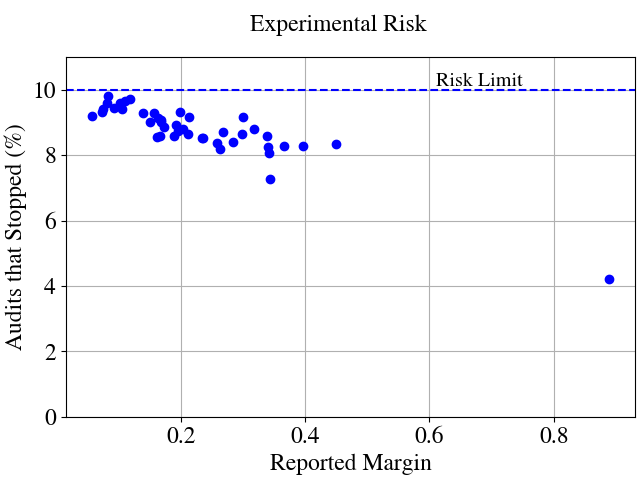
\includegraphics[width=.5\textwidth]{prov_risk.png}
\caption{The fraction of simulated \Providence audits on tied elections that stopped in any rounds (we performed five rounds at a $10\%$ risk limit). This value is an estimate of the maximum risk of the \Providence audit.}
\label{fig:prov-risk}
\end{figure}

In the simulations of \Providence audits of a tied election, the fraction of audits that stop, as shown in Figure~\ref{fig:prov-risk}, is an estimate of maximum risk. For all margins, this estimated maximum risk is less than the risk limit, supporting the claim that \Providence is risk-limiting.

\begin{figure}
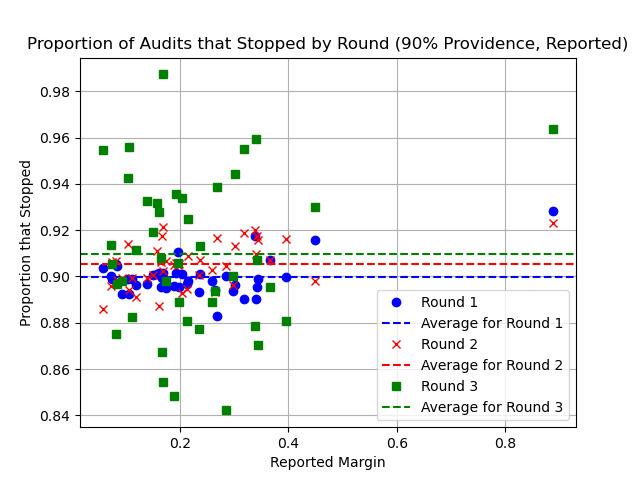
\includegraphics[width=.5\textwidth]{prov_sprob.png}
\caption{The fraction of simulated \Providence audits of the election as announced that stopped for each round. This value is an estimate of the stopping probability conditioned on the sample of the previous round. The average fraction for rounds 1, 2, and 3 is $89.96\%$, $90.52\%$, and $90.98\%$ respectively. We show only the first three rounds since so few audits make it to rounds 4 and 5.}
\label{fig:prov-sprob}
\end{figure}

Simulations of audits of the election as announced provide insight into stopping probability and number of ballots drawn when the election is as announced. We wish the stopping probability to be as predicted, and the number of ballots drawn to be small. Figure~\ref{fig:prov-sprob} shows that the stopping probabilities over the first rounds are near and slightly above $90\%$ as expected since our software chose round sizes to give at least a $90\%$ conditional stopping probability.

Figure~\ref{fig:prov-asn} plots the probability of stopping as a function of the number of ballots sampled. Points above (higher probability of stopping) and to the left (fewer ballots) represent more efficient audits. As shown, \Providence has comparable efficiency to \Minerva, while both are significantly more efficient than either implementation of \BRAVO. In a contest with a narrow margin (in the 2020 US Presidential election, eight states had margins less than $3\%$) the difference in number of ballots sampled could correspond to many days of work. 
% Section~\ref{sec:workload} discusses workload in more depth.

\begin{figure}
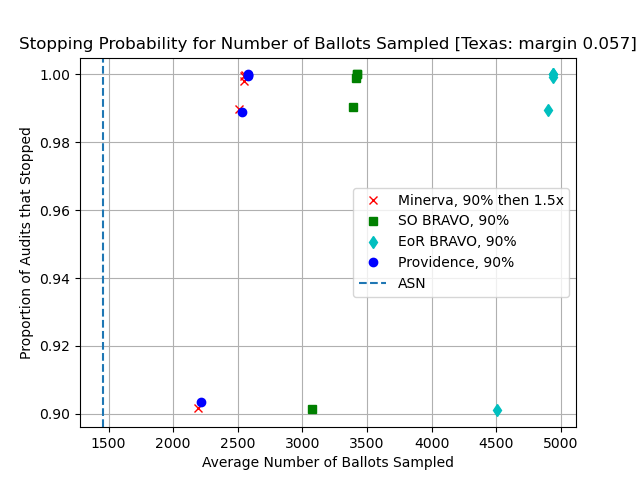
\includegraphics[width=.5\textwidth]{prov_asn.png}
\caption{For the entire audit, consisting of all five rounds, the estimated stopping probability for average number of ballots drawn for \Providence, \Minerva, EoR \BRAVO, and SO \BRAVO.}
\label{fig:prov-asn}
\end{figure}










\section{Pilot}
\label{sec:pilot}
% pilot
A pilot audit was performed in Providence, Rhode Island in February 2022 of November 2021 special elections.
The audited contest was a yes-or-no question on School Construction and Renovation Projects and had an announced $25.67\%$ margin.
The risk-limit was $10\%$.
A first round size of $140$ ballots with large probability of stopping ($95\%$) was selected, and selection order was tracked, in order to give the potential for more interesting analysis afterwards. 
As expected, the audit concluded in the first round with a \Providence risk of $4.18\%$. Table~\ref{tab:pilot-risks} shows risk measures for the drawn sample using \Minerva and \BRAVO (both EoR and SO).

\begin{table}
\begin{center}
\begin{tabular}{ |c|c|c|c|c| } 
\hline
%\diagbox[dir=NW]{First \\Round \\Size}{RLA}
ballots& \rotatebox{45}{\Providence} & \rotatebox{45}{\Minerva} & \rotatebox{45}{EoR \BRAVO} & \rotatebox{45}{SO \BRAVO} \\
\hline
140 & \bf{4.18\%} & \bf{4.18\%} & \bf{5.41\%} & 36.6\% \\
\hline
\end{tabular}
\end{center}
\caption{Risk measures for the drawn first round of $140$ ballots in the Providence, RI pilot audit. Risks in bold meet the risk-limit ($10\%$) and thus correspond to audits that would stop.}
\label{tab:pilot-risks}
\end{table}

TODO: Add examples of how the audits perform for various hypothetical round schedules. I wait to do this until I'm done with the workload estimates since the examples here should be chosen to motivate that section.


\section{Conclusion}
\label{sec:conc}
%Conclusions
A rigorous tabulation audit is an important part of a secure election. Ballot polling RLAs are commonly used and simple, not relying on special election equipment like comparison RLAs. We present \Providence which is the most efficient and secure ballot polling RLA, as efficient as \Minerva  and flexible as \BRAVO. We present proofs and simulation results to verify the claimed properties of \Providence, and we provide an open source implementation of the stopping condition and useful related functionality.





%-------------------------------------------------------------------------------
%\section{Introduction}
%%-------------------------------------------------------------------------------
%
%A paragraph of text goes here. Lots of text. Plenty of interesting
%text. Text text text text text text text text text text text text text
%text text text text text text text text text text text text text text
%text text text text text text text text text text text text text text
%text text text text text text text.
%More fascinating text. Features galore, plethora of promises.
%
%%-------------------------------------------------------------------------------
%\section{Footnotes, Verbatim, and Citations}
%%-------------------------------------------------------------------------------
%
%Footnotes should be places after punctuation characters, without any
%spaces between said characters and footnotes, like so.%
%\footnote{Remember that USENIX format stopped using endnotes and is
%  now using regular footnotes.} And some embedded literal code may
%look as follows.
%
%\begin{verbatim}
%int main(int argc, char *argv[]) 
%{
%    return 0;
%}
%\end{verbatim}
%
%Now we're going to cite somebody. Watch for the cite tag. Here it
%comes. Arpachi-Dusseau and Arpachi-Dusseau co-authored an excellent OS
%book, which is also really funny~\cite{arpachiDusseau18:osbook}, and
%Waldspurger got into the SIGOPS hall-of-fame due to his seminal paper
%about resource management in the ESX hypervisor~\cite{waldspurger02}.
%
%The tilde character (\~{}) in the tex source means a non-breaking
%space. This way, your reference will always be attached to the word
%that preceded it, instead of going to the next line.
%
%And the 'cite' package sorts your citations by their numerical order
%of the corresponding references at the end of the paper, ridding you
%from the need to notice that, e.g, ``Waldspurger'' appears after
%``Arpachi-Dusseau'' when sorting references
%alphabetically~\cite{waldspurger02,arpachiDusseau18:osbook}. 
%%
%It'd be nice and thoughtful of you to include a suitable link in each
%and every bibtex entry that you use in your submission, to allow
%reviewers (and other readers) to easily get to the cited work, as is
%done in all entries found in the References section of this document.
%
%Now we're going take a look at Section~\ref{sec:figs}, but not before
%observing that refs to sections and citations and such are colored and
%clickable in the PDF because of the packages we've included.
%
%%-------------------------------------------------------------------------------
%\section{Floating Figures and Lists}
%\label{sec:figs}
%%-------------------------------------------------------------------------------
%
%
%%---------------------------
%\begin{figure}
%\begin{center}
%\begin{tikzpicture}
%  \draw[thin,gray!40] (-2,-2) grid (2,2);
%  \draw[<->] (-2,0)--(2,0) node[right]{$x$};
%  \draw[<->] (0,-2)--(0,2) node[above]{$y$};
%  \draw[line width=2pt,blue,-stealth](0,0)--(1,1)
%        node[anchor=south west]{$\boldsymbol{u}$};
%  \draw[line width=2pt,red,-stealth](0,0)--(-1,-1)
%        node[anchor=north east]{$\boldsymbol{-u}$};
%\end{tikzpicture}
%\end{center}
%\caption{\label{fig:vectors} Text size inside figure should be as big as
%  caption's text. Text size inside figure should be as big as
%  caption's text. Text size inside figure should be as big as
%  caption's text. Text size inside figure should be as big as
%  caption's text. Text size inside figure should be as big as
%  caption's text. }
%\end{figure}
%%% %---------------------------
%
%
%Here's a typical reference to a floating figure:
%Figure~\ref{fig:vectors}. Floats should usually be placed where latex
%wants then. Figure\ref{fig:vectors} is centered, and has a caption
%that instructs you to make sure that the size of the text within the
%figures that you use is as big as (or bigger than) the size of the
%text in the caption of the figures. Please do. Really.
%
%In our case, we've explicitly drawn the figure inlined in latex, to
%allow this tex file to cleanly compile. But usually, your figures will
%reside in some file.pdf, and you'd include them in your document
%with, say, \textbackslash{}includegraphics.
%
%Lists are sometimes quite handy. If you want to itemize things, feel
%free:
%
%\begin{description}
%  
%\item[fread] a function that reads from a \texttt{stream} into the
%  array \texttt{ptr} at most \texttt{nobj} objects of size
%  \texttt{size}, returning returns the number of objects read.
%
%\item[Fred] a person's name, e.g., there once was a dude named Fred
%%%  who separated usenix.sty from this file to allow for easy
%%  inclusion.
%%\end{description}
%%
%%\noindent
%%The noindent at the start of this paragraph in its tex version makes
%it clear that it's a continuation of the preceding paragraph, as
%opposed to a new paragraph in its own right.
%
%
%\subsection{LaTeX-ing Your TeX File}
%%-----------------------------------
%
%People often use \texttt{pdflatex} these days for creating pdf-s from
%tex files via the shell. And \texttt{bibtex}, of course. Works for us.
%
%%-------------------------------------------------------------------------------
%\section*{Acknowledgments}
%%-------------------------------------------------------------------------------
%
%The USENIX latex style is old and very tired, which is why
%there's no \textbackslash{}acks command for you to use when
%acknowledging. Sorry.
%
%%-------------------------------------------------------------------------------
\section{Availability}
\Providence is implemented in the R2B2 software library for \R and \B audits.
%%-------------------------------------------------------------------------------
%
%USENIX program committees give extra points to submissions that are
%backed by artifacts that are publicly available. If you made your code
%or data available, it's worth mentioning this fact in a dedicated
%section.
%
%-------------------------------------------------------------------------------
\bibliographystyle{plain}
\bibliography{audits.bib}

%%%%%%%%%%%%%%%%%%%%%%%%%%%%%%%%%%%%%%%%%%%%%%%%%%%%%%%%%%%%%%%%%%%%%%%%%%%%%%%%
\end{document}
%%%%%%%%%%%%%%%%%%%%%%%%%%%%%%%%%%%%%%%%%%%%%%%%%%%%%%%%%%%%%%%%%%%%%%%%%%%%%%%%

%%  LocalWords:  endnotes includegraphics fread ptr nobj noindent
%%  LocalWords:  pdflatex acks
